\documentclass{article}

\usepackage{amsmath}
\usepackage{graphicx}
\usepackage[caption=false]{subfig}
\usepackage{siunitx}
\usepackage{cleveref}
\usepackage{todonotes}

\begin{document}

\section{Introduction}

In recent years, governments have spearheaded numerous initiatives to support people with disabilities and enable them to play a more active role in modern society.
The UK's Royal National Institute of Blind People (RNIB) for example has prioritised improving access to everyday services and products, such as public transport and mobile apps~\cite{rnib2016uk}.
Improvements in modern computing have made it possible for new and innovative solutions to these problems to come to the fore.
In particular, researchers in the active vision field have have made much progress in enabling machines to autonomously manipulate cameras to gather information about an environment for mapping and object finding tasks~\cite{bajcsy2018revisiting,lock2019active}.
There is, however, a significant research question about whether techniques from active machine vision can be applied to humans, i.e.\ can a machine identify a point of interest in a scene and direct a human, instead of an electronic servo, to focus on that point?
If this can be done, it would be beneficial to people with visual impairments and will augment their ability to search for an arbitrary point or object of interest and identify an unknown scene. 

The ActiVis\footnote{https://lcas.github.io/ActiVis/} project aims to deliver a mobile guidance system that will ultimately be able to guide a user with vision impairments on the last leg of their journey, i.e.\ the so-called `last 10-yard problem'. 
The prototype platform is based on a Google Project Tango\footnote{https://en.wikipedia.org/wiki/Tango\_(platform)} device, pictured in \cref{fig:tango} and \cref{fig:tango-headphone}, that embeds a colour camera and provides access to powerful real-time localisation (through IMU measurements and landmark tracking) and image-processing facilities. 
It also provides access to Android's full range of interface tools and I/O options. 
Furthermore, a set of bone-conduction headphones (pictured in \cref{fig:tango-headphone}), which are placed on a user's cheekbones instead of their ears and do not interfere with normal hearing, are used to transmit the audio signals to the user.

\begin{figure}[t]
  \centering
  \subfloat[]{\label{fig:tango}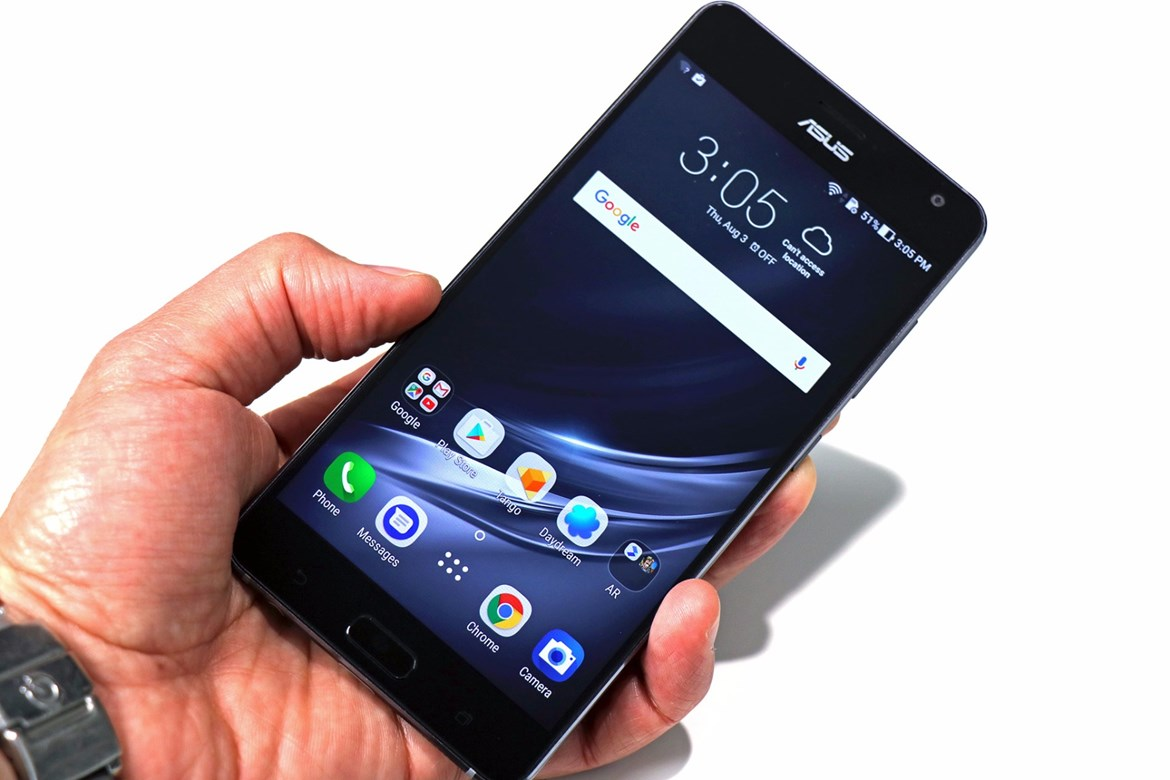
\includegraphics[width=0.4\columnwidth]{figures/tango_asus.jpeg}}
~
  \subfloat[]{\label{fig:tango-headphone}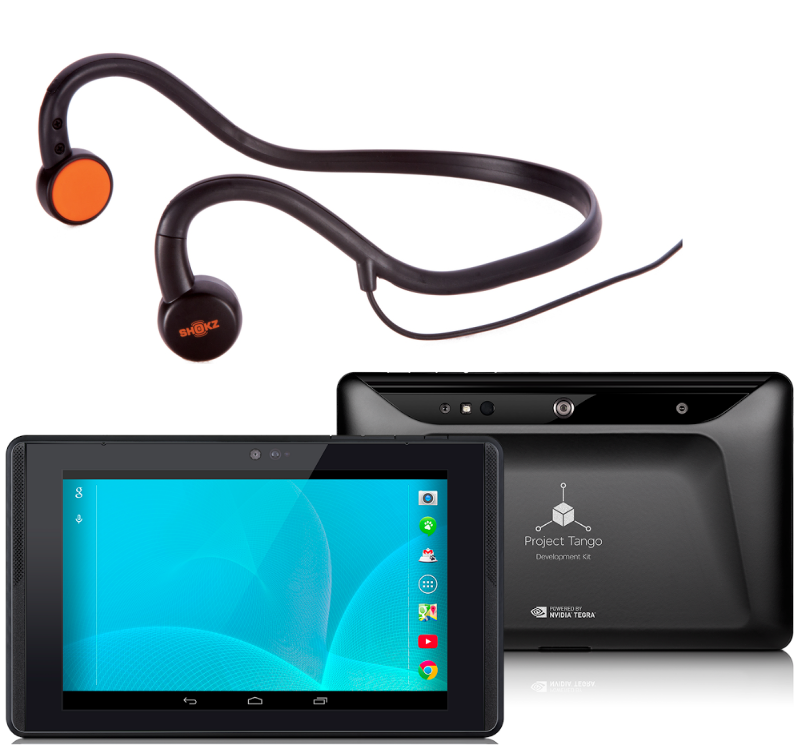
\includegraphics[width=0.3\columnwidth]{figures/tango_headphone.png}}
~
  \subfloat[]{\label{fig:participant}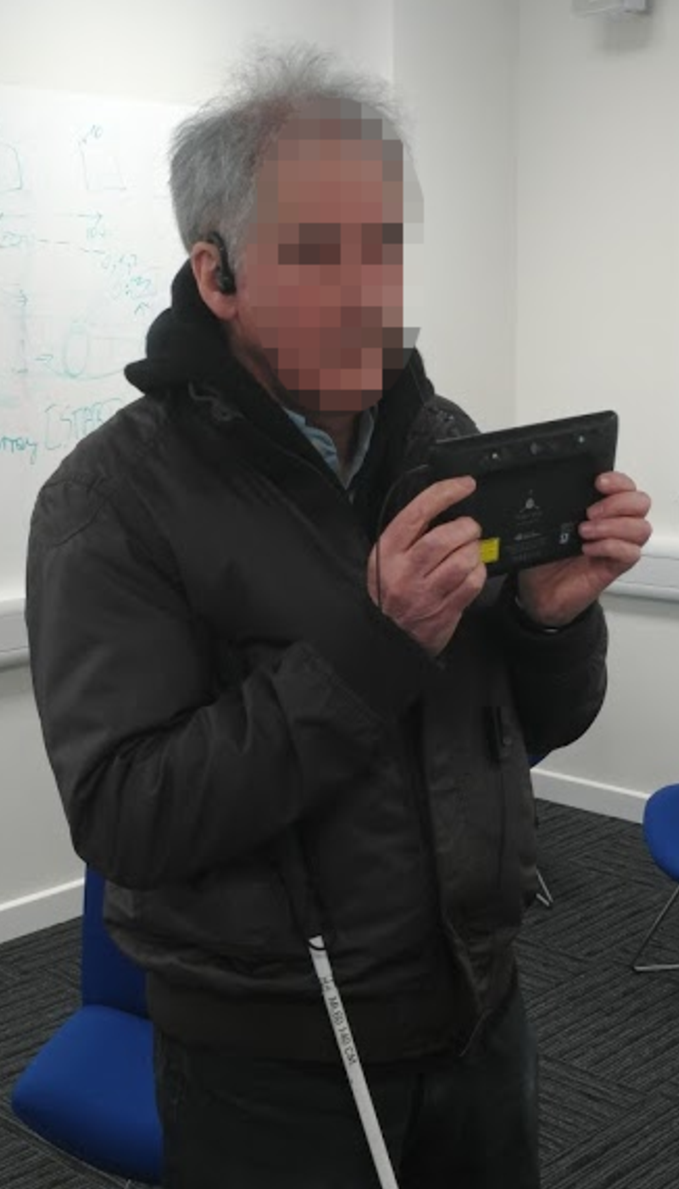
\includegraphics[width=0.2\columnwidth]{figures/vi_participant.pdf}}
  \caption{Pictures of the latest Tango mobile phone (left), the former Tango tablet and the bone-conduction headphones used in this work (centre), and a participant with visual impairments during an experiment (right).}
\end{figure}

Humans are able to determine the 3D position of a sound source and by exploiting this natural ability, the real-time guidance instructions can easily be interpreted without posing a significant cognitive load.
A sound source can be spatialised by adjusting a tone's spectral make-up (elevation angle), time delay and level difference (pan angle), and intensity (distance).
In our case, only the pan and elevation positions are transmitted to the user to point the camera towards a target object or visual feature.
However, since bone-conduction headphones bypass the outer ear structure, their spectral signature cannot properly be interpreted and we therefore convey the target's elevation angle by adjusting the tone's pitch.
A similar approach was used in~\cite{durette2008visuo} and further investigated in~\cite{lock2019bone}.
However, in this work we expand the scope and investigate the perception limitations of the interface in order to find some design guidelines and we expand the pool of participants to more than 50 people.

The rest of the paper starts by discussing previous relevant works and research in \cref{sec:prev-work}, followed by a discussion on the design and implementation of our interface in \cref{sec:system-description}.
This is followed by a description of the experiments that were conducted and a discussion of their results in \cref{sec:experiments} and \cref{sec:results}.
Finally, the paper concludes with a summary and a short discussion on future research prospects in \cref{sec:conclusion}.

\section{Previous Work}\label{sec:prev-work}

\section{System Description}\label{sec:system-description}

Existing electronic navigation aids have typically struggled to gain market traction and replace the traditional walking cane as the standard assistive tool for people with visual impairments.
Current technological limitations include prohibitive costs, bulky hardware requirements and non-user-friendly interfaces~\cite{golledge2004stated,yusif2016older,arditi2013user}.
To address these issues, we implemented a handheld mobile system that is based on a concept proposed in~\cite{lock2017portable,lock2019active} and tested in~\cite{lock2019bone} that uses a Google Tango device that is able to localise itself in real-time.
This system has the benefit of minimal hardware requirements and a compact, familiar form-factor, which will help to overcome the hurdle of user-acceptance and usability.

A set of bone-conduction headphones is used as the audio transmission medium.
These headphones sit on a user's cheekbones and conduct the audio signals through the skull into the inner ear, instead of through the outer part like typical over-ear headphones. 
This has the benefit of allowing the user access to ambient sounds and noise, so a person with limited vision can still relies on sound to detect, for example, oncoming vehicles and people~\cite{lichtenstein2012headphone}.
Alternative solutions, such as open-back headphones, were also considered.
These allow ambient noise through, but they still filter the incoming sound.
The AfterShockz headphones (\cref{fig:tango-headphone}) were ultimately selected since they do not interfere on other sounds and are also more discreet than the larger over-ear headphones. 

\subsection{Audio Interface}

Humans localise a sound source in 3 dimensions by considering cues recorded in one ear (monaural cues) and comparing cues received at both ears (binaural cues)~\cite{blauert1997spatial,blauert1969sound}.
The binaural cues include inter-aural time and level differences (ITD and ILD respectively) that help to determine a source's location on the horizontal plane.
Monaural cues are taken from the interaction of the sound with the human anatomy, e.g.\ head, shoulders, outer ear, before it enters the ear canal.
When the modified audio signal enters the inner ear canal, the human brain is able to analyse the frequency response and accurately determine the position of the sound source on the median plane. 
The distance to the source is simply derived as the intensity, or volume, of the source, i.e.\ a louder sound would appear closer to the user than a softer one. 

When an audio signal is transmitted via a set of speakers or headphones, it can be transformed with an HRTF to mimic the characteristics of a natural sound source before it is transmitted, tricking the brain into believing a sound is located at some arbitrary position.
An HRTF is a mathematical function that simulates the response signal of a human head and is derived by capturing key characteristics that affect the monaural and binaural responses, such as the user's hearing levels and head size.
Since hearing responses are unique amongst different users, the best results would be observed if each user had their own customised HRTF.\
However, given the complicated process involved to capture the required user characteristics, making unique HRTFs is often an untenable solution and using average values (e.g.\ head measurements, height, etc.) have shown to produce acceptable results~\cite{gardner1995hrtf}.

The guidance information is presented to the user in terms of pan and elevation angles, indicating the angular adjustments required to point the device camera at the target location, as shown in \cref{fig:cam-coords}.
Spatialised audio signals are well-suited to the task, displaying similar levels of performance to vocal feedback, but with less cognitive load and higher resolution~\cite{klatzky2006cognitive}.
However, given the previously discussed limitations of bone-conduction and spatialised audio, we propose a simple linear adjustment to the signal's pitch as a function of the elevation angle. 
The pan angle, instead, can be conveyed by transforming the audio signal with an HRTF, and indeed it has been found that this dimension is unaffected by using bone-conduction headphones\cite{schonstein2008comparison,macdonald2006spatial,stanley2006lateralization}. 

\begin{figure}[t]
  \centering
  \subfloat[]{\label{fig:cam-coords}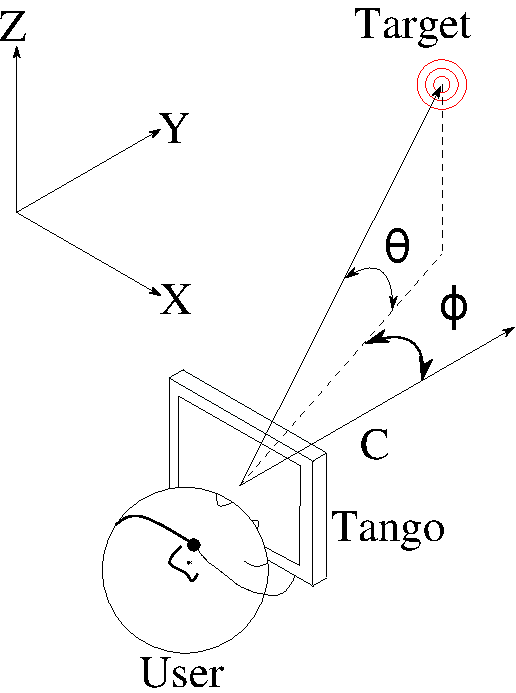
\includegraphics[width=0.3\columnwidth]{figures/camera_coordinate.pdf}}
~
  \subfloat[]{\label{fig:pitch-gain}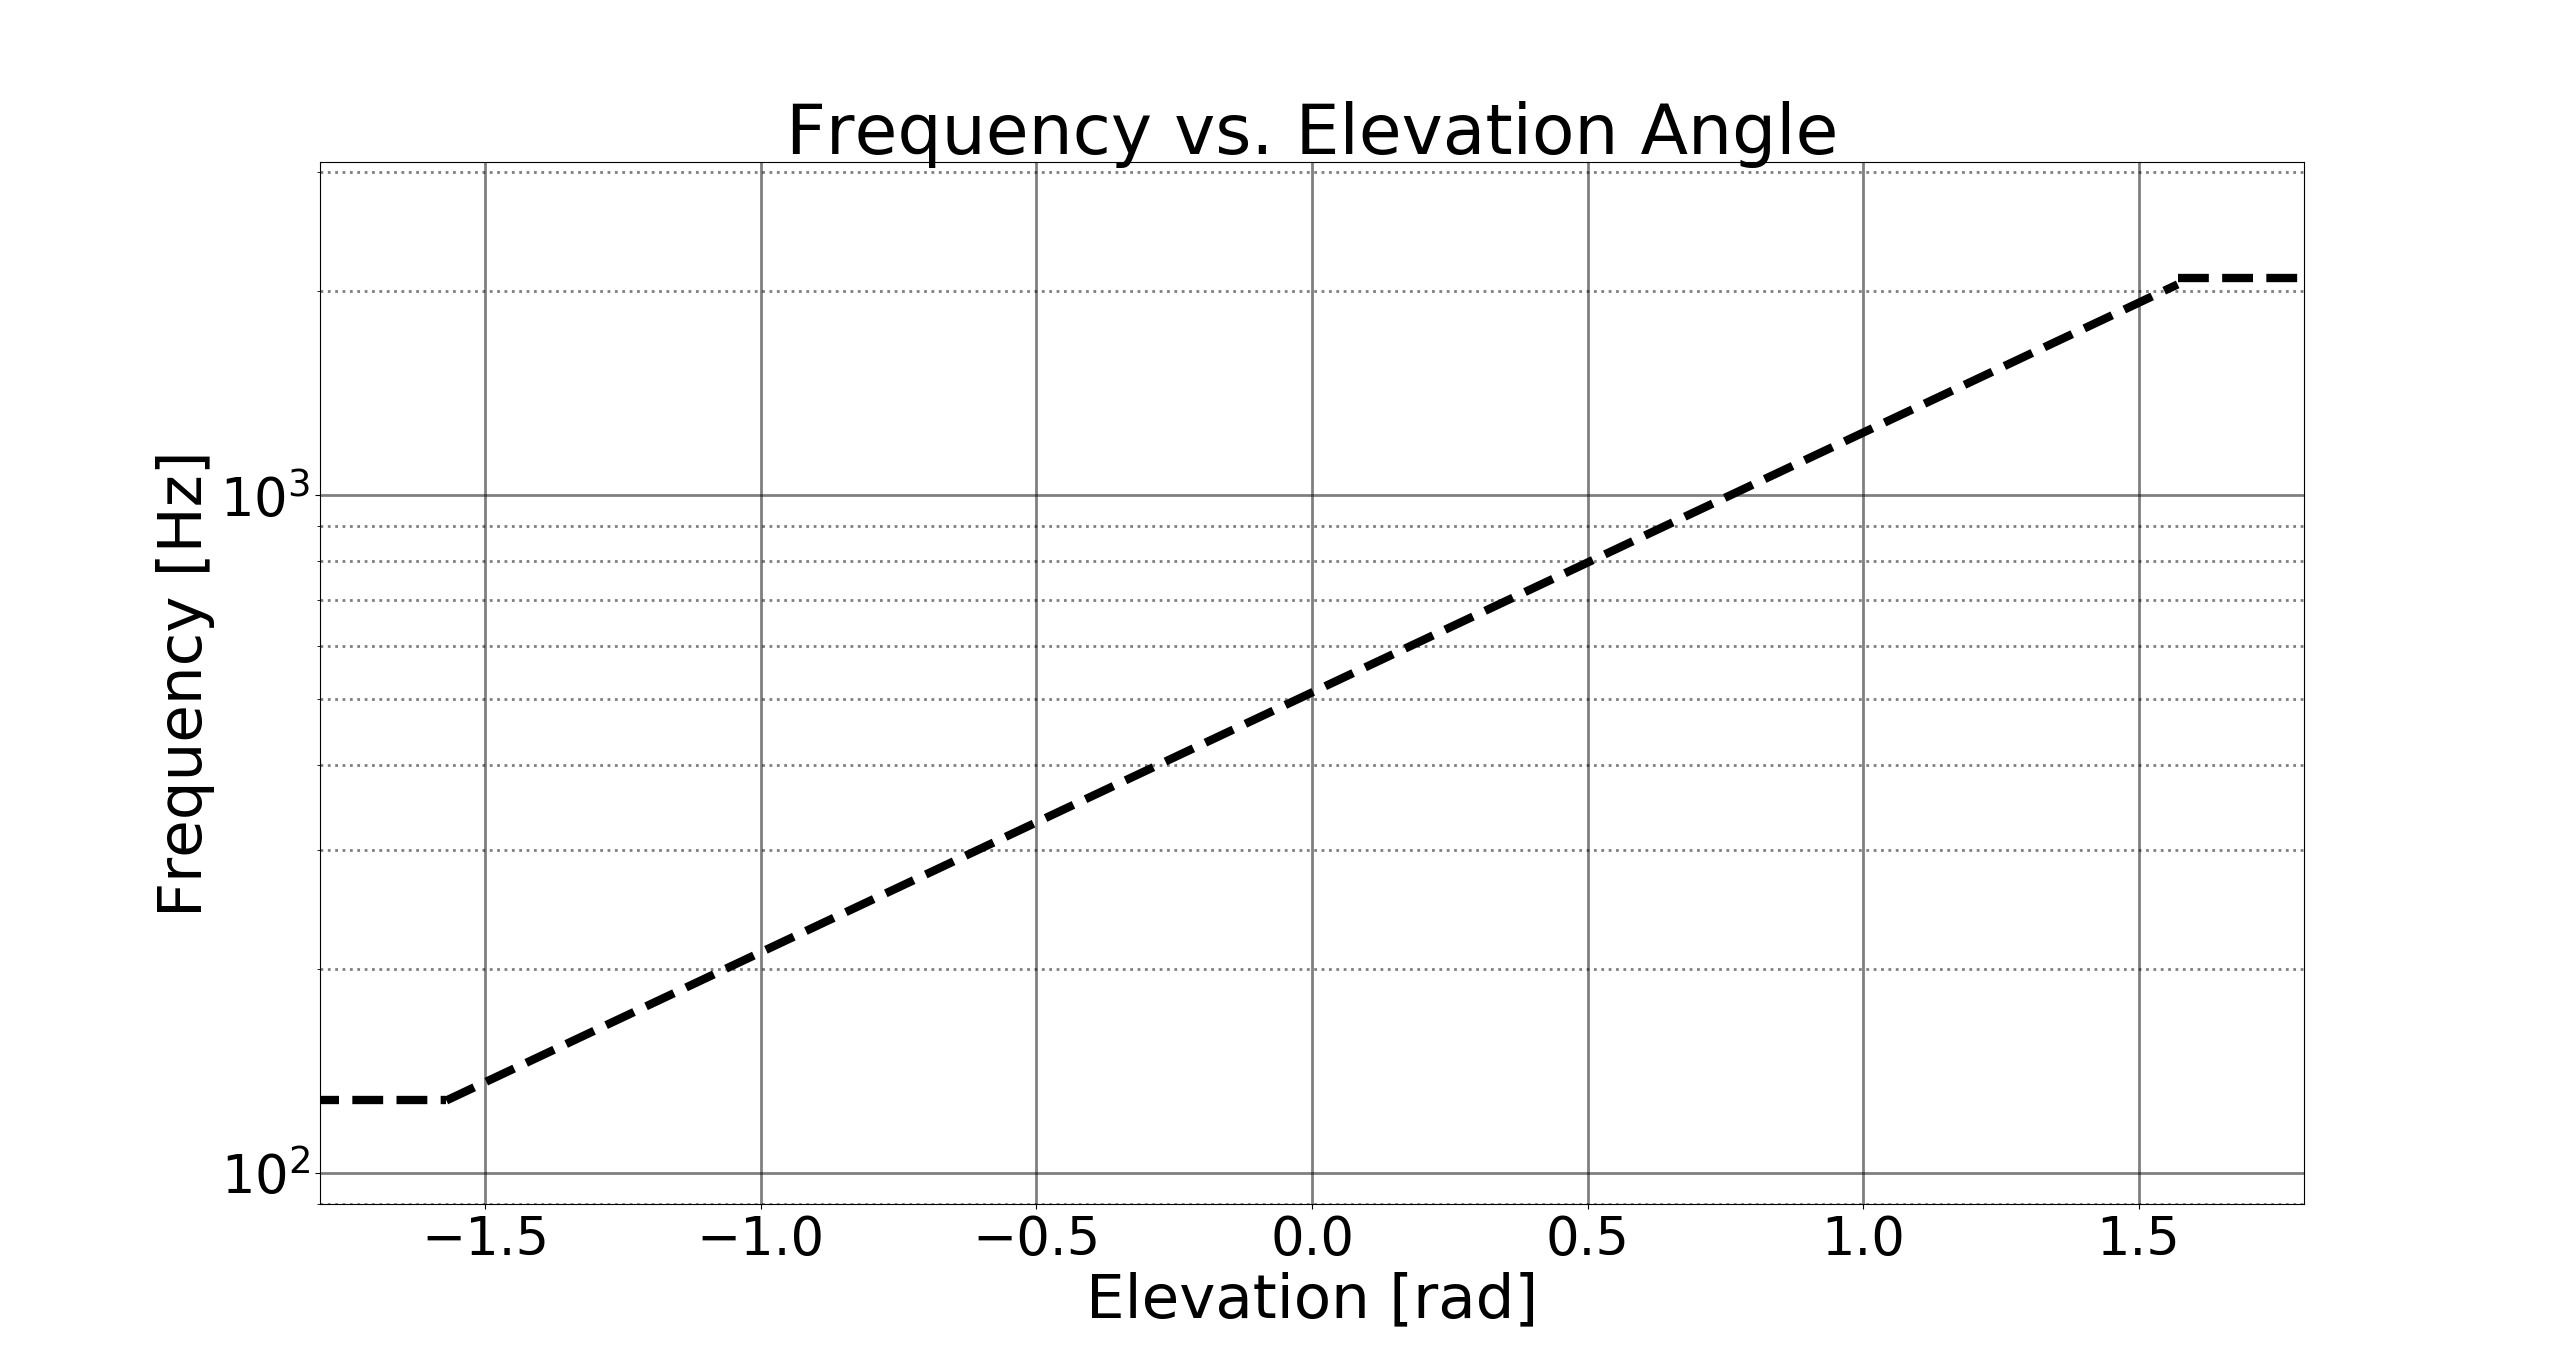
\includegraphics[clip, trim=0 0 0 40, width=0.6\columnwidth]{figures/pitch_gain_function.png}}
  \caption{The reference system used by the guidance interface showing the camera vector and pan and elevation angles (left) and the pitch gain function used to convey the target's elevation angle (right). Note the logarithmic scale of the frequency axis.}
\end{figure}

\subsubsection{Pan Dimension}

The human audition system uses binaural comparison cues, such as ITD and ILD, to localise a sound source on the horizontal plane~\cite{blauert1969sound}.
The ITD is the perceived time delay between the signal reaching both ears, while the ILD is the perceived volume difference in the signal.
For example, a sound that comes from the individual's right will hit the right ear first with a slightly higher volume.

In this work, a pure sinusoidal wave was used. 
People typically have trouble localising a pure tone without a sufficiently rich spectral signature.
However, the ITD and ILD are independent of the tone's spectral make-up, while the elevation angle is given through a different mechanism. Therefore, a pure sine wave is suitable to convey the target's pan angle.
To transform and spatialise the audio signal, we used OpenAL's default HRTF, based on the MIT's KEMAR dataset~\cite{hiebert2005openal}, which uses the person and targets' positions as input, and outputs a transformed audio signal.

\subsubsection{Elevation Dimension}

A generic HRTF implementation with bone-conduction headphones is not very effective in conveying the elevation angle of a sound source~\cite{macdonald2006spatial,schonstein2008comparison}.
To compensate for this, we communicate the target's elevation angle by adjusting the tone's pitch (i.e.\ the sine wave's frequency) as a function of the elevation. 
When the camera vector is at the correct elevation, the tone pitch is set to neutral.
When the target is above or below the camera vector, the pitch is increased or decreased, respectively.
This high/low association scheme is motivated by humans' natural association of high-pitched sounds with elevated sound sources, and low-pitched sounds with source's below the individual's earline~\cite{pratt1930spatial,blauert1997spatial}.
An octave- and semitone-based function is used to adjust the tone's pitch to ensure perceptible changes, while keeping the timbre roughly constant~\cite{shepard1964circularity}.
The pitch is updated at a rate of \SI{10}{\hertz} and changes as the user moves the device.

The pitch is changed as a linear function of the elevation angle and the gradient is determined by setting the angle and pitch limits.
For this work, we only consider a \SI{180}{\degree} field of view in front of the user and limit the elevation angle to a range of \SI{\pm90}{\degree}, or $[-\frac{\pi}{2}, \frac{\pi}{2}]$.
The pitch limits are set at some integer number of octaves above and below the neutral, on-elevation pitch.
After practical tests with the interface, we set the neutral pitch to \SI{512}{\hertz}, which is comfortably audible and allows for a large number of suitable octave limits to be selected.
We set the pitch limits to 2 octaves away from the neutral pitch, giving frequency limits of [\SI{128}{\hertz}, \SI{2048}{\hertz}].
The linear function is visualised in \cref{fig:pitch-gain}.

\section{Experiments}\label{sec:experiments}

\subsection{Implementation}

A diagram of the experimental system pipeline is shown in \cref{fig:pipeline}, where the arrows indicate the direction of the information flow.
When the user taps the Tango's screen, a new virtual target is generated and its coordinates are sent to the audio generation module, along with the device's current position and orientation.
The audio generator then produces a tone based on the difference between the device and the target's positions. The tone is sent to the audio output channel, which plays it back to the user.
A WiFi recording module is constantly monitoring the different values of the device's parameters and of the target's position, as well as the system's output, recording everything to a remotely stored datafile. 

\begin{figure}[t]
  \centering
  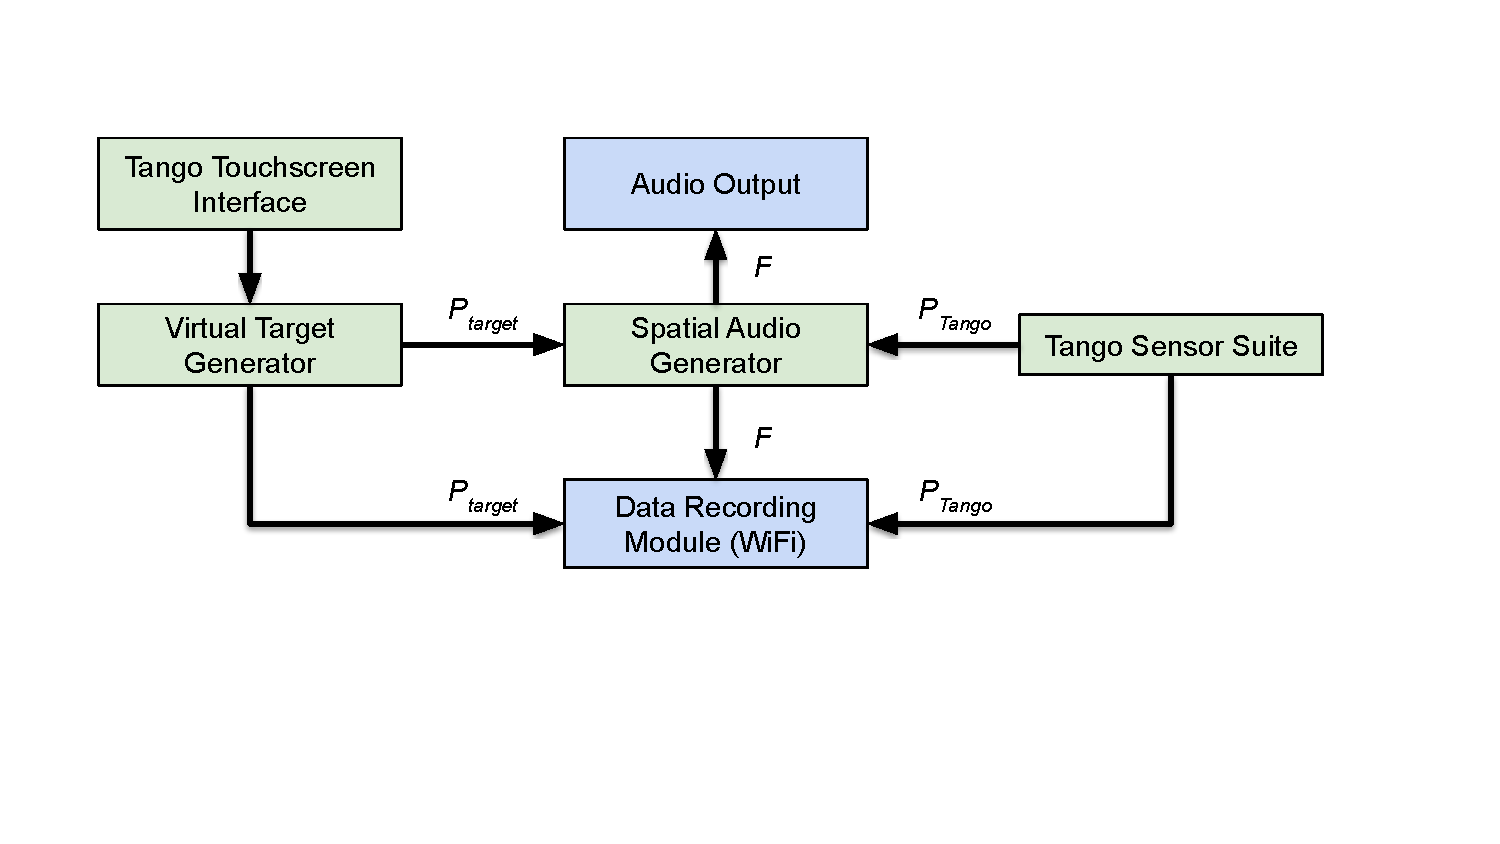
\includegraphics[clip=true, trim=0 120 80 50, width=0.9\columnwidth]{figures/pipeline.pdf}
  \caption{A diagram of the individual system components and their communication pipelines. $F$ indicates a feedback signal and $P$ a pose signal. }\label{fig:pipeline}
\end{figure}

\subsection{Participant Characterisation}

In addition to the target searching experiment, another set of experiments were conducted to characterise the participants' hearing characteristics.
The characteristics that were measured were each participant's audio localisation ability on the lateral plane, as well as the participants' ability to discriminate between tones with different frequencies. 
These results will be used to provide context to the results captured during the target search experiment and provide additional insight on any possible biases or limitations. 

\subsubsection{Sound Localisation}

In this experiment, we evaluated a participant's ability to determine the lateral direction a sound is coming from.
To do this, we played a continuous \SI{512}{\hertz} sinusoidal tone to the participant through the headphones and applied an HRTF to spatialise and place its source to the participant's left or right.
The participant then had to select the direction the sound came from.
The longer the experiment lasts and the more correct guesses the participant makes, the closer the source moves to the centre-front of the participant, making it progressively harder to localise. 

For this progressive increase in difficulty, a 2-up, 1-down step process is used~\cite{wetherill1965sequential,levitt1971transformed}, meaning that for every 2 correct answers, the distance to the centre halves.
Conversely, the task becomes easier for each incorrect answer by doubling the sound source's distance from the centre.
We also use 2 different step sequences, one starting at a large distance (\SI{45}{\degree}) from the user and the other at the minimum distance (approximately \SI{1}{\degree}), giving an `easy' and a `hard' progression respectively.
The terminating condition for the experiment is when the 2 sequences converge to within 2 intervals of one another for 3 consecutive guesses.
This gives a distance band within which the participant is capable of localising the sound source.
Each participant performed this experiment three times. 

\subsubsection{Pitch Discrimination}

Here we determined a participant's ability to differentiate the pitches of 2 tones being played to them, i.e.\ how well they can tell if a tone is high or low pitched.
We played 2 tones to the participants in succession with the second tone being higher or lower-pitched than the first.
The participants were then asked to select whether they interpreted the second tone as higher or lower-pitched than the first.

The first tone is randomly generated, while the second tone is generated by adding or subtracting some value from the first one.
The tone difference depends on how well the participant can tell the tones apart.
Like the sound localisation experiment, a 2-up, 1-down step process is used: for every 2 consecutive correct answers, the pitch difference between the tones is halved and is doubled for every incorrect answer.
2 step sequences are again used here, one starting with a large pitch difference ($f_h=2^9=$ \SI{512}{\hertz}) between the tones and the other with a small difference ($f_l=2^1=$ \SI{2}{\hertz}).
The termination condition is when the 2 step sequences are within 1 octave of each other (i.e.\ $\log_2\frac{f_h}{f_l}=2^1$) for 3 consecutive answers.
Each participant performed this experiment twice. 

\subsection{Target Search}

To test the interface's effectiveness at guiding the user in a pointing task, a set of experiments were conducted to capture the difference between the targets' actual direction and the directions the participants' perceived them to be.
The participants were given a Tango device running an app written for the experiment that generates a set of virtual targets and presents them to each participants, one at a time. 
The targets are generated at a constant distance from the participant and their pan and elevation angles are uniformly generated across the four quadrants of the pan-elevation plane to avoid clustering.
Each target's angular position is communicated to the participant through the audio interface, the output of which is adjusted in real-time as the participant points the device around. 
When a participant was confident that the device was on-target, i.e.~hearing the audio front-on at \SI{512}{\hertz}, they tapped the screen, marking the location and generating the next target.
The targets' positions are all set relative to the device's coordinate system, which is tracked using the Tango hardware and localisation API.\
A total of 28 targets were generated per participant. 

\subsection{Metrics}

We use two different metrics to compare the three different pitch gradient settings: the acquisition accuracy and search time.
The accuracy is given as the difference between the Tango's orientation at the time the participant confirmed they were on target, and the target's actual orientation.
We separate the results of the tilt and pan dimensions in order to see how the different pitch gradients affect a participant's pointing accuracy. 

We also compare the performance of the three pitch gradient settings in terms of the time it takes each participant to find a target.
However, since each participant was presented with a different, randomly generated set of targets, a direct time comparison is not possible.
Instead, we use Fitts's Law~\cite{fitts1954information}, modified by MacKenzie for uncertain target sizes and noisy data~\cite{mackenzie1992fitts}, which states that there is a relation between the time it takes to find a target and its index of difficulty (the ratio between the distance to the target and its width).
It also provides a so-called `index of performance' that we can use as a metric to compare the results between the three configurations. 

Here we briefly summarise the equations and quantities involved in our metric.
Fitts's Law is given by  

\begin{equation}
  \label{eq:fitts-base}
  t = a + bID,
\end{equation}

\noindent
where $t$ is the time it takes to find a target, $a$ and $b$ are constants determined through regression and $ID$ is a description of the difficulty of the target, given as logarithmic function of the ratio between the distance to the target and the target's width.
In our case, the targets have no width, since they are points in space, and we therefore use MacKenzie's modified form for $ID$, given by

\begin{equation}
  \label{eq:fitts-id}
  ID = \log_2\left(\frac{\theta}{w_e} + 1\right).
\end{equation}

\noindent
Here $\theta$ is the angular distance between subsequent target centres and $w_e$ is the targets' effective angular width~\cite{welford1968fundamentals}, given by

\begin{equation}
  \label{eq:fitts-we}
  w_e = \sqrt{2\pi e}\sigma = 4.133\sigma,
\end{equation}

\noindent
where $\sigma$ is the standard deviation of the error data, taken as the angle between the participant's target selection and target's actual angular position.
Fitts's index of performance, $IP$, can then be calculated using 

\begin{equation}
  \label{eq:fitts-performance}
  IP = \frac{ID}{t},
\end{equation}

\noindent
where $IP = \frac{1}{t}$ when $\sigma=0$.

\subsection{Procedure}

Two groups of participants were recruited for the experiments on a volunteer basis. 
Group \textit{G1} consisted of 42 young adults with normal eyesight who were blindfolded for the experiments, and group \textit{G2} contained 10 people with severe visual impairments (18-55 years old, 40 female, 16 female). 
None of the participants had any hearing or other disabilities that could have influenced their performance in the experiments.
Each participant performed 3 sets of experiments each, with the 2 characterisation experiments preceding the final target-search experiment. 
Both groups were given some time before the experiment target-search experiment to familiarise themselves with the system, the audio signal's behaviour and the \SI{512}{\hertz} on-level tone. 
Furthermore, to minimise the speed/accuracy biases in the results for this experiment, we asked the participants to focus on finding the targets, without worrying about the time it took. 

\section{Results}\label{sec:results}

\subsection{Sound Localisation}

\cref{fig:sound-localisation} shows the results captured from the sound localisation experiment where the participants had to select the direction (left or right) that the tone was being played to them from. 

\begin{figure}
  \centering
  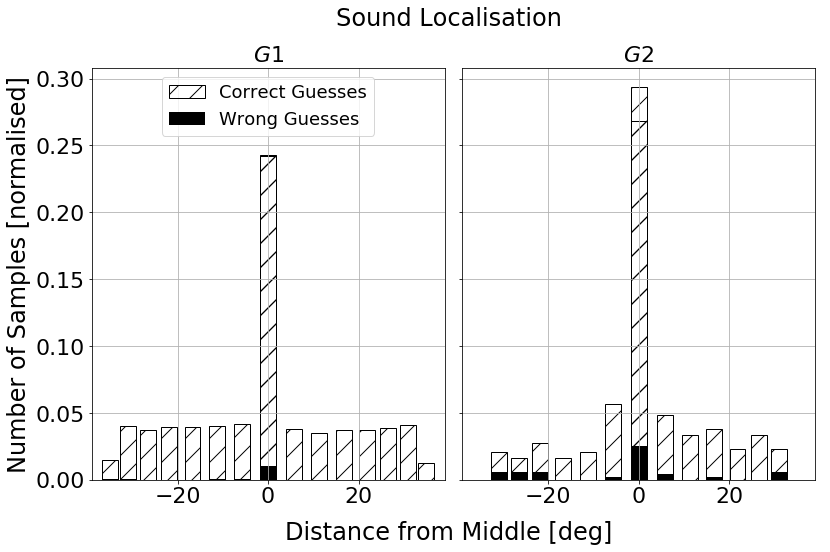
\includegraphics[width=1.0\textwidth]{figures/sound_localisation.png}
  \caption{Histograms of the participants' guesses of the tone locations that show the correct and incorrect guesses for each bin. }
  \label{fig:sound-localisation}
\end{figure}

From inspection of \cref{fig:sound-localisation}, it can be seen that the vast majority of guesses for both groups were correct.
For Group \textit{G1}, the majority of erroneous guesses were made at the minimum distance from the centre, i.e.\ the most difficult to guess correctly, which is the expected behaviour and indicates that the participants consistently progressed through the distance intervals.
We can therefore conclude that the participants from \textit{G1} had little difficulty determining sound direction.

Group \textit{G2} also displays a concentration of erroneous guesses in the centre interval.
However, it also has more incorrect guesses in other distance intervals and displays a more even progression through the distance intervals towards the centre.
This could indicate that instead of terminating the experiment through bringing the 2 sequences within 1 interval of one another, there was more switching back and forth between the centre 3 intervals. 

These results show that both participant groups are capable of determining a sound source's location with a reasonable level of consistency and accuracy
These results are in line with what we expected and are supported by literature which indicates that humans are very adept at localising a sound source, particularly in the pan dimension. 

\subsection{Pitch Discrimination}

The results of the pitch discrimination experiment are shown in \cref{fig:pitch-discrimination} where bar plots are used to show the proportion of correct to incorrect guesses of which tone was higher pitched for different tone difference intervals. 
The latter is given in terms of semitone differences which is obtained with 

\begin{equation*}
\label{eq:semitone-difference}
  \Delta f = 12\log_2\frac{f_0}{f_1}.
\end{equation*}

For Group \textit{G1}, we see that their guesses are normally spread around the 0 semitone difference interval and as expected, the highest proportion of incorrect guesses occur in the $[-0.25, 0.25]$ semitone difference interval. 
The guesses from Group \textit{G2} is more concentrated around the centre and the majority of incorrect guesses also occurs in the $[-0.25, 0.25]$ semitone difference interval.

Assuming the differences are normally spread, we fitted a cumulative distribution function (CDF) over each participant's set of results for their correct guesses.
We then used each CDF's parameters to determine a frequency threshold where the participant could not longer reliably tell the tones apart. 
The threshold is set to contain 75\% of each participant's correct guesses and an example of one participant's threshold can be seen in \todo{put in figure}.
The median of these threshold values can then be used to estimate the frequency difference at which the participant population could no longer tell the difference between two tones and can be used to improve the next interface iteration's frequency profile and increase performance. 
\cref{fig:pitch-thresholds} shows a distribution of the thresholds values for each group, along with the median value. 
The median is used here given the skewed plot and was found to be approximately 0.4 semitones for each group.

\begin{figure}
  \centering
  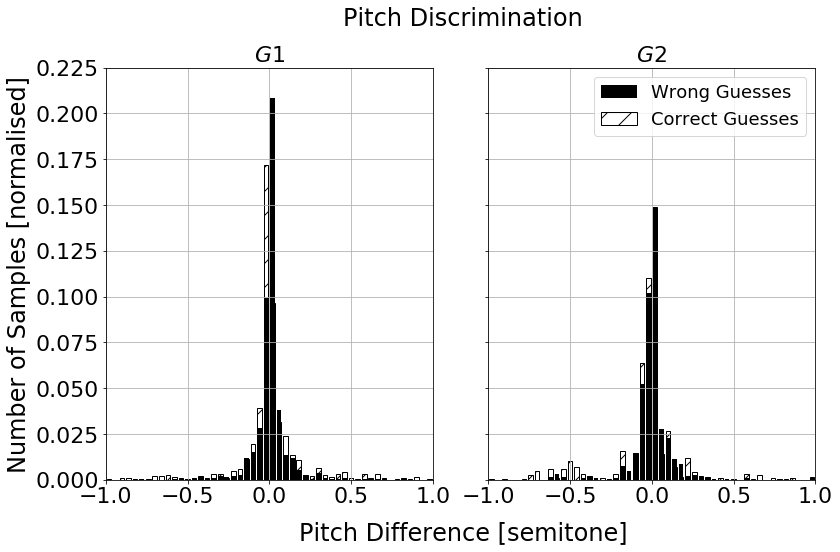
\includegraphics[width=1.0\textwidth]{figures/pitch_discrimination.png}
  \caption{Histograms of the participants' guesses of which tone was higher pitched that show the correct and incorrect guesses for each bin. }
  \label{fig:pitch-discrimination}
\end{figure}

\begin{figure}
  \centering
  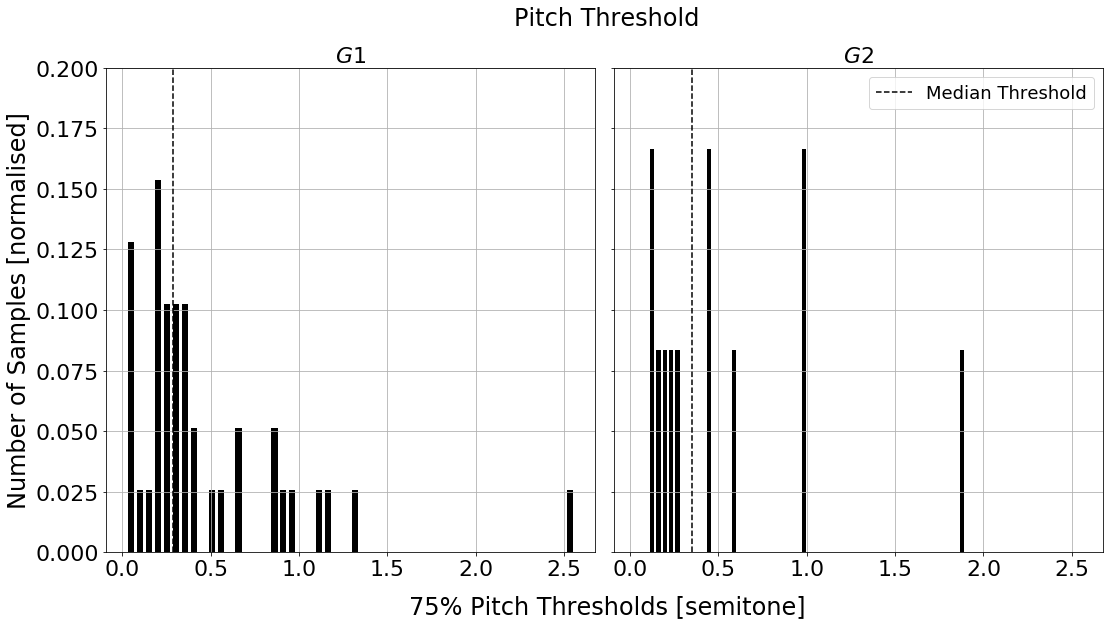
\includegraphics[width=1.0\textwidth]{figures/pitch_thresholds.png}
  \caption{Distributions of the median cut-off frequency thresholds along with the median 75\% cut-off thresholds. }
  \label{fig:pitch-thresholds}
\end{figure}

\begin{figure}
  \centering
  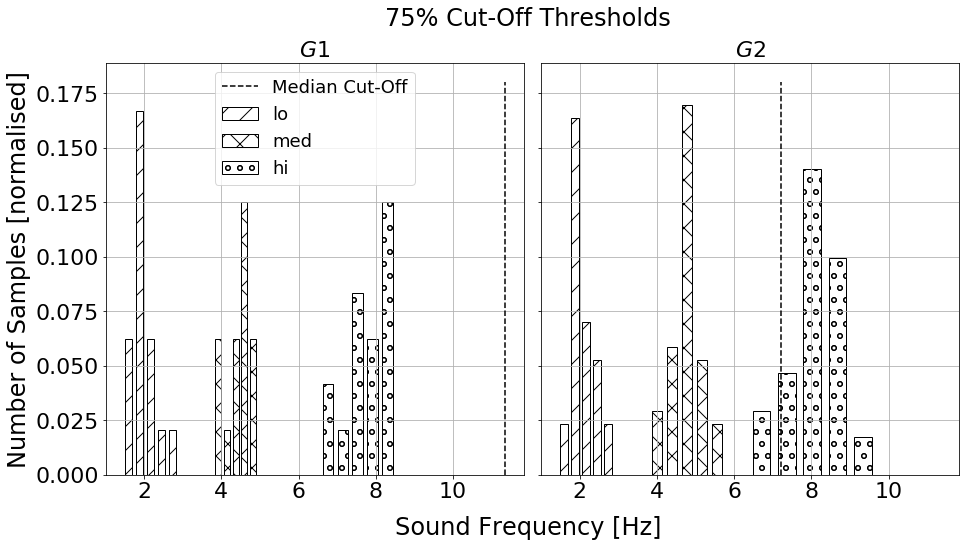
\includegraphics[width=1.0\textwidth]{figures/pitch_thresholds_limits.png}
  \caption{Histrogram distibutions of the participants' 75\% cut-off thresholds. }
  \label{fig:pitch-thresholds-hist}
\end{figure}

\subsection{Target Search}

The results from the target search experiment in the pan dimension are given on the abscissa of the 2D histograms in \cref{fig:target-errors}, where the angular errors in the pan and tilt directions are plotted against each other. 
A set of box-plots of the pan errors are also given in \cref{fig:target-boxplot-error} for each audio setting.
The results are summarised in \cref{tab:target-results}\todo{tabulate results}.

\begin{figure}
  \centering
  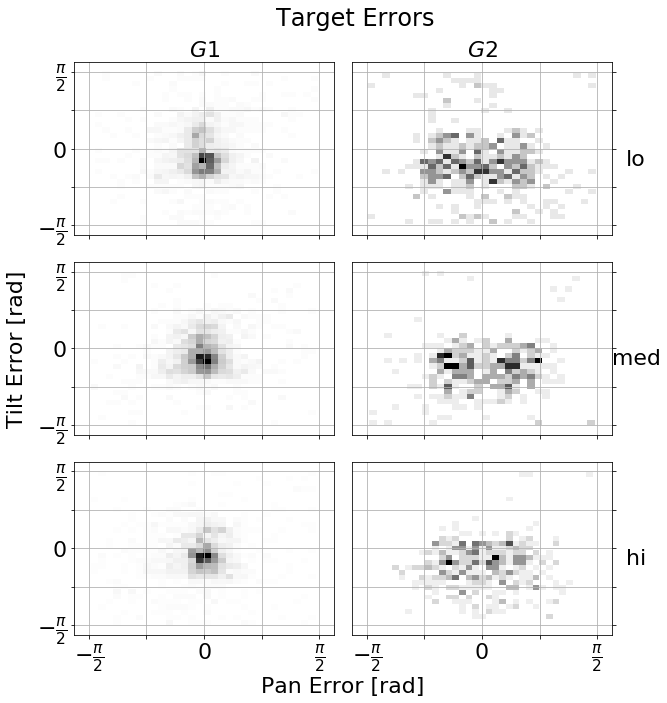
\includegraphics[width=1.0\textwidth]{figures/target_errors.png}
  \caption{Distributions of the angular errors in the pan and elevation dimensions for the 3 different pitch gradient settings. }
  \label{fig:target-errors}
\end{figure}

The Shapiro-Wilkes test for normality reveals that none of these distributions are normally spread and accordingly, the Pearson test is used to investigate the correlation between the actual target location and participants' pointing location.
These results are included in \cref{tab:target-results}.
The Pearson correlation scores for Group \text{G1} indicate a moderate to strong positive correlation between the target and the selected locations ($r_{pan} \in [0.71, 0.76], p < 0.001; r_{elevation} \in [0.36, 0.48], p < 0.001$), showing that the both the pan and elevation cues roughly worked as expected.
However, the correlation scores for Group \textit{G2} are significantly weaker, with a pan angle correlation of $r_{pan} \in [0.2, 0.48], p < 0.001$.
The elevation correlation is somewhat stronger, with $r_{elevation} \in [0.46, 0.53], p < 0.001$.
However, the correlation score for the elevation for the \textit{lo} setting is disregarded for having insufficient statistical relevance ($p > 0.05$). 

The repeated-measures procedure that was used for these experiments required the data for each participant to be grouped together for each setting.
The medians of these groupings of error data are then used as individual samples that represent an individual participant's performance for each setting.
\cref{fig:target-boxplot-error} shows this median data collected from each participant as a set of boxplots, while \cref{fig:target-boxplot-absolute-error} shows the absolute error data for these groupings. 

\begin{figure}
  \centering
  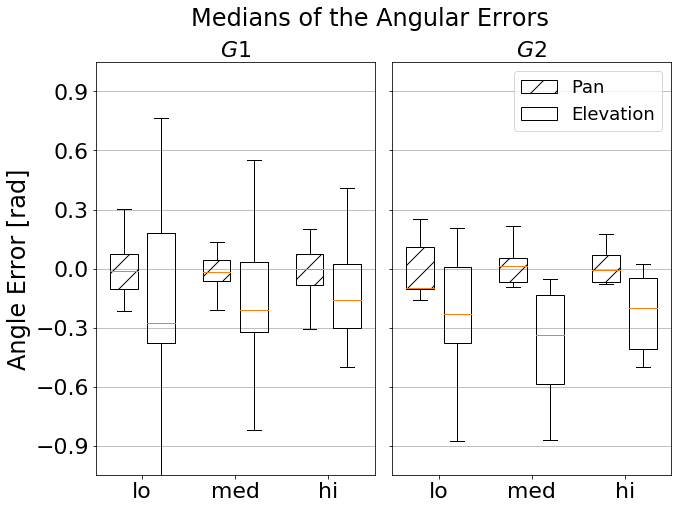
\includegraphics[width=1.0\textwidth]{figures/boxplot_target_search_median_error.png}
  \caption{Boxplots of the median pan and elevation errors for each setting. }
  \label{fig:target-boxplot-error}
\end{figure}

\begin{figure}
  \centering
  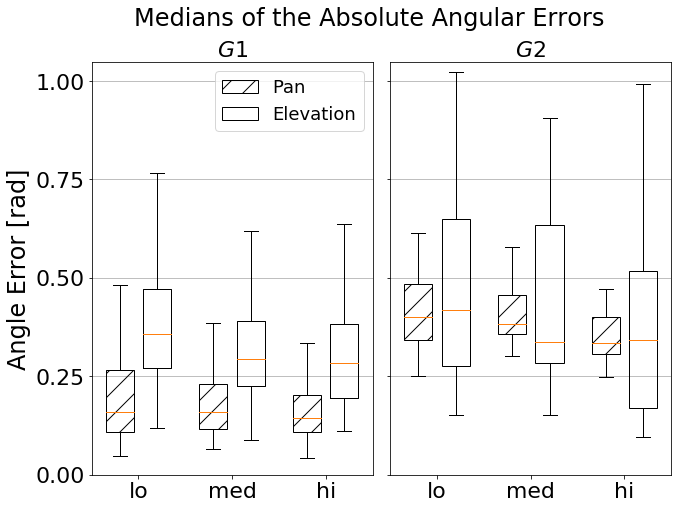
\includegraphics[width=1.0\textwidth]{figures/boxplot_target_search_absolute_median_error.png}
  \caption{Boxplots of the absolute median pan and elevation errors for each setting. }
  \label{fig:target-boxplot-absolute-error}
\end{figure}

The boxplots in \cref{fig:target-boxplot-error} shows that the error in the pan dimensions is roughly centred around \SI{0}{\radian} for both groups, with some divergence between the groups and settings for the different settings.
However, these divergences are determined to not be significant using the Friedman test for repeated measures ($p \gg 0.05$), showing that spatialisation perception and accuracy is not affected by changes in the tone's pitch.

Analysis of the elevation data with the Friedman test reveals that the results for the different settings within each group are indeed significantly different from one another with a reasonable degree of confidence ($p_{G1} = 0.03, p_{G2} = 0.01$).
A post-hoc analysis using the Wilcoxon signed rank test with a Holm-Bonferoni correction applied to the commonly used 0.05 statistical significance threshold was used to investigate the setting relationships more closely. 
This analysis reveals that there is only 1 significant difference between the performances generated by the \textit{med} and \textit{hi} settings for Group \textit{G1} ($p_{med-hi} = 0.002$), while Group \textit{G2} has 2 significantly different levels of performance between the \textit{lo} and \textit{med} settings, as well as for the \textit{med} and \textit{hi} settings ($p_{lo-med} = 0.011, p_{med-hi} = 0.001$).
It can also be noted that there is a significant negative error bias observed in all of the settings in both groups which is possible caused by a cognitive constraint introduced by the floor where the participants believed that the targets could not appear below the ground.
Since this bias seems constant in nature, it can be addressed by adjusting the frequency parameters of the interface and shifting it by a constant offset. 

With these results, we can reasonably conclude that the \textit{hi} setting  
The distributions in \cref{fig:target-boxplot-error} show that the \textit{hi} setting produces the smallest median angular error in the elevation dimension out of the 3 settings and the post-hoc tests performed allow us to make the conclusion that the \textit{hi} setting is indeed the best setting to produce the lowest error. 

\subsection{Time to Target}

To investigate if the interface has a Fitts-relationship, we plot the time to find the target as a function of the targets' indices of difficulty as defined in \cref{eq:fitts-base}.
The data was binned in intervals of the effective target width as given by \cref{eq:fitts-we} and are plotted for each gradient setting. 
A logarithmic line of best fit is fitted through the binned data's median values through means of regression and all the results are presented in \cref{fig:fitts-results}.

\begin{figure}
  \centering
  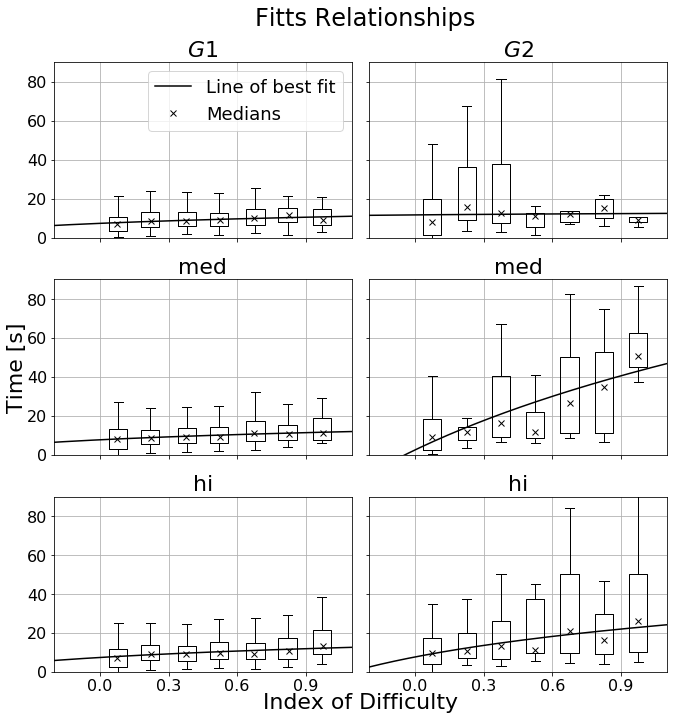
\includegraphics[width=1.0\textwidth]{figures/fitts_fit.png}
  \caption{Plots showing the Fitts relationship between the time it took the participants to find a target and the target's index of difficulty. }
  \label{fig:fitts-results}
\end{figure}

For Group \textit{G1}, a Fitts relationship can be observed where the logarithmic line of best fit closely approximates the median values of the binned data for all 3 settings. 
This is confirmed with strong Pearson correlation scores for each setting ($r_{lo} = 0.9, p_{lo} = 0.03; r_{med} = 0.92, p_{med}=0.009; r_{hi} = 0.86, p_{hi} = 0.02$).
Regarding Group \textit{G2}¸ we observe larger spreads for each binned dataset, indicating less consistency int eh time to target results for participants with severe sight impairments.
However, the results for the \textit{med} and \textit{hi} settings exhibit strong Pearson correlation scores ($r_{med} = 0.88, p_{med} = 0.019; r_{hi} = 0.89, p_{med} = 0.03$), while the results for the \textit{lo} setting does not produce a statistically significant correlation ($r_{lo} = 0.23, p_{lo} = 0.65$).

These results allows us to calculate and plot the index of performance, as given in \cref{eq:fitts-performance}, for each setting in \cref{fig:fitts-ips}.

\begin{figure}
  \centering
  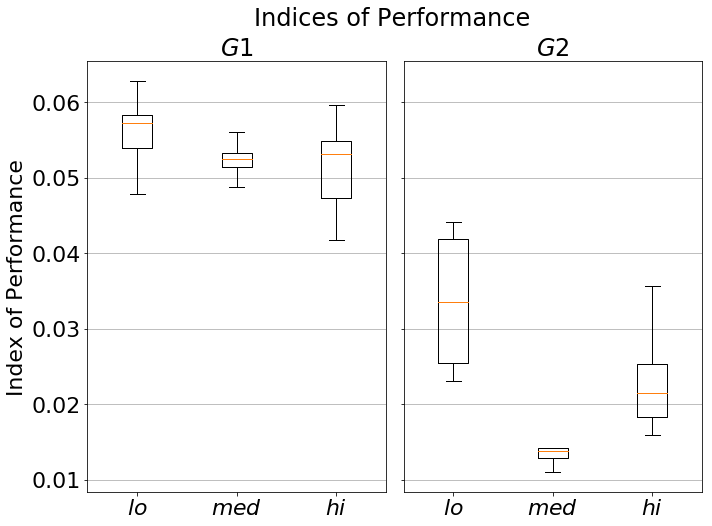
\includegraphics[width=0.7\textwidth]{figures/fitts_ips.png}
  \caption{Plots showing the Fitts relationship between the time it took the participants to find a target and the target's index of difficulty. }
  \label{fig:fitts-ips}
\end{figure}

For the results from Group\textit{G1}, there is a progressive improvement in performance between the \textit{lo}, \textit{med} and \textit{hi} settings respectively, with the \textit{hi} producing the highest level of performance between the 3 settings, i.e.\ the participants found the targets with the smallest error in the least about of time with the \textit{hi} setting.
This is supported by the results from the Friedman test ($p < 0.001$), as well as post-hoc Wilcoxon tests with Holm-Bonferroni corrections that show all 3 datasets are significantly different from one another ($p_{lo} = p_{med} = p_{hi} < 0.001$).
The results for Group \textit{G2} shows far lower indices of performance for each setting, which is expected given the increased indices of difficulty observed in \cref{fig:fitts-results}.
Indeed, the distributions are shown to be similar according to the Friedman test ($p = 0.1$) and we cannot conclude which setting produces the best performance. 
\todo{explain why bad}

A possible reason why the \textit{hi} setting produces the highest level of performance is that the higher gradient makes it easier to perceive changes in the tone's pitch for each unit change in the device's pointing direction.
The observed effect is that the \textit{hi} setting drives the user to the target location in in the least amount of time and with the highest level of accuracy. 

This trend of progressive improvement between the \textit{lo}, \textit{med} and \textit{hi} settings respectively seems indicate that that simply increasing the frequency gradient will lead to increased performance.
However, \cref{fig:pitch-thresholds-hist} indicates that the frequency difference between the on-target tone and the selected tone in the \textit{hi} setting is approaching the cut-off frequency for Group \textit{G1}, indicating the point at which increasing the gradient produces diminishing returns on performance. 
Indeed, the participants from Group \textit{G2} seems to have passed this threshold and reached a saturation point where they could no longer reliably tell changes in the tone apart any longer. 

\section{Conclusion}\label{sec:conclusion}

\bibliographystyle{plain}
\bibliography{bib}

\end{document}
